\documentclass[a4paper]{amsart}

\usepackage{color}
\usepackage[colorlinks=true, citecolor=red]{hyperref}  %needs to come before amsrefs package to work with \cite{}*{}
\usepackage{amssymb,latexsym}
\usepackage[alphabetic]{amsrefs}
\usepackage[mathscr]{eucal}
\usepackage{pdfsync}
\usepackage{graphicx}
\usepackage{epstopdf}
\DeclareGraphicsRule{.tif}{png}{.png}{`convert #1 `dirname #1`/`basename #1 .tif`.png}
\usepackage[all]{xy}
\usepackage{titletoc}
%\usepackage[show]{ed}
%\usepackage{txfonts}   %  \fint  for integral average

%\usepackage{showkeys}  %options notref  notcite 

%\input{rgb.tex}

%\textcolor{DarkRed}{text in DarkRed}


\CompileMatrices

\theoremstyle{plain}
\newtheorem{theorem}{Theorem}[section]
\newtheorem{lemma}[theorem]{Lemma}
\newtheorem{proposition}[theorem]{Proposition}
\newtheorem{corollary}[theorem]{Corollary}

\theoremstyle{definition}
\newtheorem{definition}[theorem]{Definition}%[section]
\newtheorem{assertion}[theorem]{Assertion}%[section]


\theoremstyle{remark}
\newtheorem{defn}[theorem]{Definition} 
\newtheorem{example}[theorem]{Example}
\newtheorem{remark}[theorem]{Remark}
\newtheorem{discussion}[theorem]{Discussion}

%\numberwithin{equation}{section}

%\newcommand{\abs}[1]{\lvert#1\rvert}

\DeclareMathOperator{\Lip}{Lip}
\DeclareMathOperator{\dist}{dist}
\DeclareMathOperator{\expected}{\mathbb{E}}
\DeclareMathOperator{\prb}{Prob}
\DeclareMathOperator{\spt}{spt}
\DeclareMathOperator{\lap}{\Delta}
\DeclareMathOperator{\Tr}{Tr}

\raggedbottom

\addtolength{\textwidth}{2cm}
\addtolength{\oddsidemargin}{-1cm}
\addtolength{\evensidemargin}{-1cm} 
\addtolength{\topmargin}{-1cm} 
\addtolength{\textheight}{2cm}

\newcommand{\side}[1]{\footnote{\emph{Draft Comment}:  #1}}
%\newcommand{\side}[1]{} 

\def\Xint#1{\mathchoice
   {\XXint\displaystyle\textstyle{#1}}%
   {\XXint\textstyle\scriptstyle{#1}}%
   {\XXint\scriptstyle\scriptscriptstyle{#1}}%
   {\XXint\scriptscriptstyle\scriptscriptstyle{#1}}%
   \!\int}
\def\XXint#1#2#3{{\setbox0=\hbox{$#1{#2#3}{\int}$}
     \vcenter{\hbox{$#2#3$}}\kern-.5\wd0}}
\def\ddashint{\Xint=}
\def\dashint{\Xint-}




%%% BEGIN DOCUMENT
\begin{document}

\title{Axiom of Choice, Zorn's lemma and Well Orderings}  
\author{John E.\ Hutchinson}
\date{\today}




\maketitle
``The Axiom of Choice is obviously true, the well-ordering principle obviously false, and who can tell about Zorn's lemma?''   Jerry Bona

``The Axiom of Choice is necessary to select a set from an infinite number of socks, but not an infinite number of shoes.''   Bertrand Russell


\tableofcontents



We will see that the axiom of choice,  the well ordering principle and  Zorn's lemma each imply one another.  We follow  the treatment in~\cite{Dud}*{pp 12--15, 18--21}. 

In particular, the following surprising results are true.
\begin{itemize} 
\item There is a well ordering of the real numbers and of $ \mathbb{R}^n  $ for any $ n $.  
\item Every vector space has a basis in the linear algebra sense.  For example, 
\begin{enumerate}
 

\item There is a  a set of continuous functions 
\[ 
S \subset \mathcal{C} (\mathbb{R} ) := \{ f : \mathbb{R} \to \mathbb{R} \mid f \text{ is continuous}\},
\]
such that every $ f \in \mathcal{C} (\mathbb{R} )$ can be written uniquely as a finite sum of the form
\[
   f = \sum_{i=1}^n a_i \phi_i 
   \]
   for some $ n \geq 1 $, $ a_i \in \mathbb{R} $ and $ \phi_i \in S $.
   
   \item For any Hilbert space $ \mathcal{H} $ there is a set $ S \subset \mathcal{H} $ such that every $ f \in \mathcal{H} $ can be written uniquely as a finite sum of the form
\[
   f = \sum_{i=1}^n a_i \phi_i 
   \]
   for some $ n \geq 1 $, $ a_i \in \mathbb{R}\ (\text{or }\mathbb{C} ) $ and $ \phi_i \in S $.
   
   
\item There is a set $ S \subset \mathbb{R} $  such that every $ x \in \mathbb{R}$ is a unique finite linear sum 
\[
x = \sum_{i=1}^n r_i y_i 
\]
   for some $ n \geq 1 $, $ r_i \in \mathbb{Q}   $ and $ y_i \in S $.
\end{enumerate} 
\end{itemize} 
 


%%%%%%%%%%%%%%%%%%%%%%%%%%%%%%%%
%%%%%%%%%%%%%%%%%%%%%%%%%%%%%%%%
%%%%%%%%%%%%%%%%%%%%%%%%%%%%%%%%
%%%%%%%%%%%%%%%%%%%%%%%%%%%%%%%%
\section{\textbf{Preliminaries}} 

\begin{definition}
 $ (X,\leqslant) $ is a \emph{partial ordering} if $ \leqslant $ is a binary relation on $ X $ such that 
\begin{enumerate}
\item $ a\leqslant b $ and $ b \leqslant c $ implies $ a \leqslant c $  (transitive),
\item $ a \leqslant a $ (reflexive),
\item $ a \leqslant b $ and $ b \leqslant a $ implies $ a=b $  (antisymmetric).
\end{enumerate} 
We write $ a < b $ if $ a \leqslant b $ and $ a \neq b $.
\end{definition}

\begin{example} \label{expo} The following are partial orderings.

\begin{enumerate}

\item For any set $ X $, $( \mathcal{P} (X), \subset )$ (where ``$ \subset $'' allows equality of sets).
\item   An example we will use later is, with $ V $  a vector space, the partial ordering $ (X,\subset) $ where
\[
X = \{ S \subset V \mid \text{every finite subset of $ S $ is linearly independent}\}.
\]

\item The usual $ \leqslant $ ordering on $ \mathbb{Z} $, $ \mathbb{N} $ or $ \mathbb{R} $.
\item $ X = \{ a,b,c,d,e,f,g\} $ with the partial ordering described in Figure~\ref{pd}. 
\end{enumerate} 

 \begin{figure}[htbp] %  figure placement: here, top, bottom, or page
    \centering
    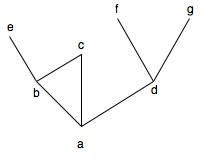
\includegraphics[width=2in]{pd.jpg} 
    \caption{$ x \leqslant y $ if $x=y $ or  there is a ``rising'' path from $ x $ to $ y $.   For example,  $ a \leqslant b $, $ a \leqslant c $ and $ a \leqslant e$.}
    \label{pd}
 \end{figure}
  \end{example}
  
  
\begin{definition}
$ (X,\leqslant ) $ is a \emph{linear ordering} if it is a partial ordering such that
$ a,b \in X  $ implies $ a \leqslant b $ or $ b  \leqslant a $ (note both are true precisely when $ a=b $).

%
 $ L \subset X $ is an \emph{initial segment} of $ X $ if ($ y\in L\ \&\ x < y) \Longrightarrow  x \in L $. 

 \end{definition}
 
\begin{example} Only (3) in Example~\ref{expo} is a linear ordering.
\end{example} 
 
  
\begin{definition}
If $ (X,\leqslant )$ is a  partial ordering then $a  \in X $ is a \emph{maximal} element if there is no $ b $ such that $ a < b $. We say $ a $ is a \emph{greatest} element if $ b \leqslant a $ for every $ b \in X$.   
\end{definition}


\begin{remark}\mbox{}

\begin{enumerate}
\item There is at most one greatest element in a partial ordering.  
\item Every greatest element is a maximal element.
\item  In Figure~\ref{pd} the maximal elements are $e,c,f,g $.  There is no greatest element. 
\item An important example is $ (X, \subset ) $ from (2) in Example~\ref{expo}.
We say that $ S \subset V $ is a \emph{basis} for $ V $ if $ S \in X $ (i.e.\  if every finite subset of $ S $ is   linearly independent), and if every $ v\in V $ is a \emph{finite} linear combination of elements from $ S $.%
\footnote{An orthonormal basis in the Hilbert space sense is \emph{not} a basis in this sense.  Here we are defining a basis in the usual algebraic sense, sometimes called a Hamel basis --- there is no notion of a limit.

It follows $ S \in X $ is maximal iff $ S $ is a basis for $ V $ \emph{Why?}.

An orthonormal base in a separable Hilbert space is countable.  A basis is always uncountable. \emph{Exercise}.}
\end{enumerate}
\end{remark}
  
 \begin{definition} $ (X,\leqslant ) $ is a \emph{well ordering} if it is a linear ordering such that every non-empty subset of $ X $ contains a least element.%
 \footnote{A \emph{least} element of $ A \subset X $ is of course an element $ a \in A$ such that $ a \leqslant b $ for all $ b \in A $.}
   \end{definition}

 \begin{example} \label{woex}\mbox{}
   
\begin{enumerate}
 \item The only example of a well ordering in Example~\ref{expo} is $ \mathbb{N} $  in (3).
   \item  $X =  \mathbb{N}\cup \{a\} $     is a well ordering if we use the standard ordering on $ \mathbb{N} $ and set $ n < a $ for all $ n \in \mathbb{N} $.  
  \item $ \mathbb{N} $ followed by another copy of $ \mathbb{N} $  is a well ordering.
  \item Many more examples can be constructed this way.
 \end{enumerate}
 \end{example}
 
 
\begin{definition} Suppose $(X,\leqslant ) $ is a well ordering.

 The \emph{first} or \emph{initial} element is the least element of $ X $.
 
 If $ x \in X $ is any element then its \emph{successor} is the least element $ y $ such that $ x<y $, and is denoted by $ s(x) $.  Thus $ s(x) $ exists  unless $ x $ is the greatest element of $(X,\leqslant ) $. 

 A \emph{successor} element is an element of the form $ s(x) $.
 
 
 A \emph{limit} element $ x\in X $ is an element which is not the first element and not a successor element.  Equivalently, $ x $ is not the first element and for every $ y < x$  there is an element $ z $ such that $ y < z < x $.
 \end{definition}

  
  In Example~\ref{woex}(3) the ``first'' 1 is the initial element. The ``second'' 1 is a limit element.  All other elements are successor elements.
 
    
  
\begin{proposition} If $ (A,\leqslant) $ and $ (B,  \preccurlyeq ) $ are well orderings then  one is isomorphic to an initial segment (perhaps all) of the other.
\end{proposition}
 
 \begin{proof}
We don't need the result, and the proof is like that for the following Proposition.  So I leave it as an exercise.
  \end{proof} 
 
 
We often define a function by induction over the natural numbers by first defining $ f(1) $ and then defining $ f(n) $ in terms of $ f(1),\dots, f(n-1) $.  For example, the Fibonacci sequence is defined by
\[  
f(1)=1, \ f(2) =1, \ f(n) = f(n-2) + f(n-1) \text{ for } n \geq 3.
\]

In  general, we can define 
\[
f(n) = g \big(f \lfloor I(n)\big),
\]
where $ g $ is a given function, $ I(n)$ is the initial segment $   \{k : k < n \} $, and $ f \lfloor I(n) $ is the restriction of $ f $ to $ I(n) $. 

It is useful here to think of a function as a set of ordered pairs, so   $f \lfloor I(n) = \{ (k,f(k)) : k < n\} $.
 
 \medskip We now generalise inductive definitions to well ordered sets.
  
\begin{proposition}[Definition by Recursion] \label{dfrec} Suppose $ (X, \leqslant ) $ is a well ordered set.  Let $ I(x) = \{ y : y < x \} $ for each $ x \in X $.  Then given $ g $ with range $ T $ and appropriate domain, there is a unique function $ f :X\to T $ such that 
\begin{equation} \label{dr} 
 f(x) = g \big(f \lfloor I(x)\big).
\end{equation} 
\end{proposition} 

\begin{proof} The idea is straightforward.  

Let $ J(x) = \{ y : y  \leqslant x \} $.%
\footnote{It is very convenient  to work with initial segments of the form $J(x) $  as well as with $ I(x) $.}

Let $ G $ be the set of those $ z \in X $ such that there is   a function  of the form $ f:J(z) \to T $   which satisfies 
~\eqref{dr} for all $ x \in J(z) $.

For each $ z\in G $ there can be at most one such function.  If not, consider the first $ x \leqslant z $ where two such functions differ and obtain an immediate contradiction, since by  \eqref{dr}  they must agree at $ x $.

If $ y_1 < y_2 $ and there exist corresponding such functions $ f_1  $ and $ f_2 $, then $f_2 \lfloor I(y_1)$ is of the required form and so equals $ f_1 $. 

 It follows that $ G $ is an initial segment of $ X $.  Moreover, $ f $ is uniquely defined 
 and satisfies \eqref{dr} for all $ x \in G $.

If $ G \neq X $ let $ y $ be the least element in $ X \setminus G $.  Then we can use \eqref{dr} to extend   
$ f $ from $ G $ to $ G \cup\{y\} $. This contradicts the definition of $ G $.

Hence $ G=X  $ and we are done.
\end{proof} 

  
%%%%%%%%%%%%%%%%%%%%%%%%%%%%%%%%%%%%
\section{\textbf{Five equivalent versions of AC}} 

See Figure~\ref{AC2} for the following.
\begin{assertion} [AC: The Axiom of Choice]   Suppose $ \{S_x : x\in I \}$ is a family of non-empty sets.  Then there 
exists a function $ f $ with domain  $ I $  such that $ f(x) \in S_x $ for all $ x \in I $.
\end{assertion} 

\begin{figure}[htbp] %  figure placement: here, top, bottom, or page
   \centering
   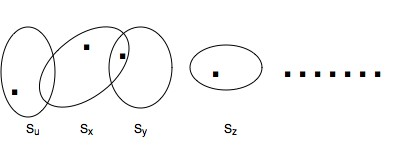
\includegraphics[width=4in]{AC2.jpg} 
   \caption{Axiom of Choice with choice function indicated by black dots.}
   \label{AC2}
\end{figure}

\begin{remark}
 \mbox{}
\begin{enumerate}

\item A function is a set of ordered pairs, and so AC asserts the existence of a \emph{set} with certain properties.  

The axiom of choice is different from most other axioms of set theory which assert the existence of a set and in effect give a rule for membership of that set.  For example, the axiom of set theory asserting the existence of the union of a family of sets, or the axiom asserting the existence of the power set of a set, gives a rule for membership of the union or power set respectively.

\item The axiom of choice as formulated above says that if $ S_x $ is non empty for every $ x \in I$ then the cartesian product $ \prod_{x\in I} S_x $ is also non empty.  So it certainly seems a very harmless axiom!  But it has some non obvious and even counter intuitive consequences, as we will see.

\item If the index set $ I $ is finite, then the axiom of choice follows from the other axioms of set theory and the rules of logic (i.e.\ first order predicate calculus). 

\item If there is a ``rule'' for selecting an object from each $ S_x $ then one does not need the axiom of choice.  For example, if $ S_x = \{0,1\} $ for each $ x $ then one can take $ f(x) = 0 $ for all $ x $, or $ f(x) = 1 $ for all $ x $.
\end{enumerate} 
 \end{remark} 


The following is a useful alternative to AC.
\begin{assertion}[AC*]  For any set $ X $ let $ I = \{A\subset X : A \neq \emptyset \}$.
Then there exists   $ f :I \to X $  such that $ f(A)\in A $ for all $ A \in I $.
\end{assertion}
 
\begin{proposition}\label{2AC}
AC is equivalent to AC*.
\end{proposition}

\begin{proof} (AC $\Longrightarrow $ AC*): AC* is the  particular case  of AC obtained by taking $ S_A = A $.

\smallskip  (AC* $\Longrightarrow $ AC): Assume AC*.  
Suppose $ \{S_x : x\in I \}$ is a family of non-empty sets.  Let $ X = \bigcup_{i\in I} S_x $. See Figure~\ref{AC}
\begin{figure}[htbp] %  figure placement: here, top, bottom, or page
   \centering
   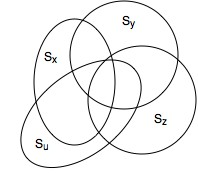
\includegraphics[width=1.8in]{AC.jpg} 
   \caption{$ X = \bigcup_{x\in I} S_x $. See Proposition~\ref{2AC}.}
   \label{AC}
\end{figure}
 
By AC*
\[ \exists g : \mathcal{P} (X) \setminus \{\emptyset\} \to X 
\text{ such that } g(A) \in A \quad  \forall A \subset X, A\neq \emptyset.
\]
Define 
\[ 
 f(x) = g(S_x) \quad \forall x \in I .
 \qedhere \]
\end{proof}


\begin{assertion}[WO: The Well-Ordering Principle]  Every set can be well-ordered.
\end{assertion}




\begin{assertion}[HMP: Hausdorff's  Maximal Principle]  Suppose   $ (X,\leqslant) $ is a partially ordered set. Then $ X $ contains a maximal linearly ordered subset.%
\footnote{$ L $ is a \emph{maximal} linearly ordered subset if it is linearly ordered by $ \leqslant $ and if there is no larger  linearly ordered subset containing $ L $.}
\end{assertion} 


\begin{assertion}[ZL:  Zorn's Lemma]  Suppose $   (X,\leqslant) $ is a partially ordered set such that every linearly ordered subset $ L $ has an upper bound in $ X $. (That is, $ \exists y \in X $ such that $ x \leqslant y $ for all $ x\in L $.)

Then $ (X,\leqslant ) $ has a maximal element.
\end{assertion}

Here are two surprising propositions which follow from ZL and WO respectively.



\begin{proposition} Every vector space $ V $ contains a basis $ S^* $.  That is,  every finite subset of $ S^* $ is linearly independent and every $v\in V $ is a unique finite linear combination of elements from~$ S^* $. 
\end{proposition}

\begin{proof}  (The point here is that this includes the case where $ V $  is not finite dimensional).

We apply ZL. (One could alternatively use HMP.)

Let $ X $ be the collection  of those $ S\subset V $ such that every finite subset of $ S $ is linearly independent.   

Then $ X $  is a partial ordering under $ \subset $.  

If $ L $ is a linearly ordered subset of $ X $ then 
$ \bigcup \{ S : S \in L \} $ is a subset of $ V $ with the property that every finite subset   is linearly independent (\emph{why?}).    Hence $ \bigcup \{ S : S \in L \} \in X$ and is an upper bound for $ L $ (\emph{why?}).

By Zorn's lemma, $ X $ has a maximal element $ S^* $  (in fact many).  Every element in $ V $ is a finite linear combination of elements of $ S^* $, as otherwise we could enlarge $ S^* $ and contradict its maximality. The fact this linear combination is unique follows from the fact every finite subset of $ S^* $ is linearly independent (\emph{why?}).  
\end{proof} 

\begin{proposition} $ \mathbb{R}^n $ can be well ordered.
\end{proposition}

\begin{proof} By the well ordering principle.
\end{proof}


%%%%%%%%%%%%%%%%%%%%%%%%%%%%%%%%
\section{\textbf{Proof of the various equivalences}}

\begin{theorem} AC $  \Longleftrightarrow$  AC* $ \Longleftrightarrow$  HMP $ \Longleftrightarrow$  ZL $ \Longleftrightarrow$  WO.
\end{theorem}

\begin{proof} We have already seen  AC $  \Longleftrightarrow$  AC*.  

We will show 
AC* $ \Longrightarrow$  WO $ \Longrightarrow$  HMP $ \Longrightarrow$  ZL $ \Longrightarrow$ AC*.

\medskip
\textbf{1}: \noindent (AC* $ \Longrightarrow$  WO):  Suppose $ f $ is a ``choice function'' satisfying $ f(A)\in A $ for all $ \emptyset \neq A \subset X $. 

 The informal idea is to define the well ordering $ x_1, x_2, \dots, x_n , \dots, x_\omega, \dots $ by
\[
x_1= f(X) , \  x_2= f(X\setminus \{x_1\}),\  x_3= f\big(X\setminus \{x_1,x_2\}\big) ,\  \dots\ ,\
  x_\omega =  f\big(X\setminus  \{x_n : n \in \mathbb{N} \}\big), \ \dots \ .
  \]
  
To make this precise consider all well orderings $ (A,\leqslant ) $ such that 
\begin{enumerate}
\item $ A\subset X$,
\item $ x\in A \Longrightarrow x = f\big(X\setminus \{ y \in A : y < x \} \big) $.
\end{enumerate} 
 We have just seen  there are indeed some such well orderings.
 
 We \emph{claim} if $ (A,\leqslant ) $ and $ (B, \preccurlyeq) $ are two such well orderings then one is an initial segment of the other (with the same ordering).   
 
 Suppose neither  $ (A,\leqslant ) $  nor $ (B, \preccurlyeq) $   is   an initial segment of the other.   
 
 Then it follows that for some $ x \in A $,  $ \{y\in A : y\leqslant x \} $%
 \footnote{It is important for the proof to take $ \{y\in A : y\leqslant x \} $ and not $ \{y\in A : y< x \} $.  Note that doing this gives  us more information, since not every initial segment is of the form  $ \{y\in A : y\leqslant x \} $.}
  is not an initial segment of $ (B, \preccurlyeq) $.%
 \footnote{Since otherwise, if $ \{y\in A : y\leqslant x \} $ is an initial segment of $ (B, \preccurlyeq) $ for every $ x \in A $, then taking the union one can check that this implies  $ A $  is an initial segment of $ (B, \preccurlyeq) $.}
 
 Take the first $ x \in A $ such that $ \{y\in A : y\leqslant x \} $ is \emph{not} an initial segment of $ (B, \preccurlyeq) $. It follows that   $ D:= \{y\in A : y< x \} $ is an initial segment of both $ (A,\leqslant ) $ and $ (B, \preccurlyeq) $.%
 \footnote{Since $ \{y\in A : y< x \} = \bigcup_{\{y\in A : y< x \}}  \{z\in A : z\leqslant  y \}$, and a union of initial segments is an initial segment.  Similarly for $ B $.}
 
 We will show $ x \in B $ and that by ``adding'' $ x $ to the end of $ D $ we get  $ \{y\in A : y\leqslant x \} $ is an initial segment of both $ A $ and $ B $, contradicting the definition of $ x $.
 
\smallskip  By property (2) for the well ordering $ (A,\leqslant) $,  we have $ x = f (X\setminus D) $.  
 
 On the other hand, since $ B\setminus D  $ is non empty (as otherwise $ B $ is an initial segment of $ A $) there is a least element $ x^* $ in $ B\setminus D  $.  Then  by property (2) for the well ordering $(B, \preccurlyeq)$,  we have $ x^* = f (X\setminus D) $. 
 
 Hence $ x^*=x $ and so by ``adding'' $ x = x^* $ to the end of $ D $ we see $ \{y\in A : y\leqslant x \} $ is an initial segment of $ (B, \preccurlyeq) $, contradicting the definition of $ x $.
 
 \smallskip Thus for any two well orderings   satisfying (1) and (2), one is an initial segment of the other.  For this reason we can take the union of \emph{all}  such well orderings to get a well ordering of some   $Y \subset  X $.  If $ Y \neq X $ then we can enlarge the well ordering by adding $ f(X\setminus Y ) $ at the end, thus contradicting the fact we took the union of all such well orderings.
 
\medskip
\textbf{2}: \noindent (WO $ \Longrightarrow$  HMP):  Suppose $ (X,\leqslant) $ is a partial  ordering and assume there is a well ordering  $(X, \preccurlyeq) $. 

The idea is to use the well ordering $ \preccurlyeq $ to build up the maximal linearly ordered subset  $ L $ for $ \leqslant $.  Let the well ordering be $ x_1, x_2, \dots, x_n, \dots, x_\omega, \dots\ $.  
Set  $ x_1 \in L $.  If $ \leqslant $ gives a linear ordering on $ \{x_1,x_2\} $ then include $ x_2 \in L $, otherwise exclude it.  If  $ \leqslant $ gives a linear ordering on $ \{x_3\} \cup \{\text{elements already in $ L $}\} $ then include $ x_3 \in L $, otherwise exclude it.  \dots \ If $ \leqslant $ gives a linear ordering on $ \{x_\omega\} \cup \{\text{elements already in $ L $}\} $ then include $ x_\omega \in L $, otherwise exclude it. Etc.

To make this precise we define $ L $, or more precisely the characteristic function $\mathcal{X}_L $,  by recursion as in Proposition~\ref{dfrec}.    That is
\[
\mathcal{X}_L(x)  = \begin{cases} 
                              1 & \text{if $ \leqslant $ is a linear ordering on $ \{ x \} \cup
                                                   \{y: y  \prec x \ \& \ \mathcal{X}_L(y) = 1\}$} \\
                               0 & \text{otherwise}
                               \end{cases}.
\]
Then $ \prec $ is a linear order on $ L $ and $ L $ is also maximal in this respect.%
\footnote{Since if $ \prec $ is a linear order on $ L\cup\{x\} $ then the definition gives $ \mathcal{X}_L(x) = 1 $, and so $ x \in L $.}
 

\medskip
\textbf{3}: \noindent (HMP $ \Longrightarrow$  ZL): Assume HMP.  

Suppose $   (X,\leqslant) $ is a partially ordered set such that every linearly ordered subset  has an upper bound in $ X $. By HMP there is a \emph{maximal} linearly ordered subset $ L $.  Let $ y $ be an upper bound for $ L $.

Then $ y $ is clearly a maximal element for $ (X,\leqslant) $.%
\footnote{Since if $y <  w $ then $ L \cup \{w\} $ would be linearly ordered, contradicting the maximality of $ L $.}


\medskip
\textbf{4}: \noindent (ZL $ \Longrightarrow$  AC*): Assume ZL.  

Given a set $ X $, let $ F $ be the set of all choice functions $ f $ whose domain is a \emph{subfamily} of the family of all non empty subsets of $ X $.  By ``choice'' function it is meant as usual that $ f(A)\in A $ for all $ A $ in the domain of $ f $.
 
Define the partial order $ \leqslant $ on $ F $ by $ f \leqslant g $ if $ g $ is an extension of $ f $.  Then it is straightforward to check that $ (F,\leqslant )$ is a partial ordering.  Moreover, any linearly ordered subset has a greatest element, obtained by taking the union (regarding a function as a set of ordered pairs) of all functions in the linearly ordered subset.  

By ZL there is a maximal element   $f \in  (F,\leqslant )$.  The domain of $ f $ must be $ \mathcal{P}(X)\setminus \{\emptyset\} $ as otherwise we could extend $ f $ by adding an ordered pair $ (x,A) $ for any non empty set $ A \subset X $ and $ x \in A $.%
\footnote{There is \emph{not} a hidden application here of AC because of our ``choosing'' $ A $ and then choosing $ x \in A $. \emph{Why?}}
\end{proof} 




%%%%%%%%%%%%%%%%%%%%%%%%%%%%%%%%
%%%%%%%%%%%%%%%%%%%%%%%%%%%%%%%%
%%%%%%%%%%%%%%%%%%%%%%%%%%%%%%%%
%%%%%%%%%%%%%%%%%%%%%%%%%%%%%%%%


\begin{thebibliography}{9} 

\bib{Dud}{book}{
   author={Dudley, R. M.},
   title={Real analysis and probability},
   series={Cambridge Studies in Advanced Mathematics},
   volume={74},
   note={Revised reprint of the 1989 original},
   publisher={Cambridge University Press},
%   place={Cambridge},
   date={2002},
   pages={x+555},
%   isbn={0-521-00754-2},
 %  review={\MR{1932358 (2003h:60001)}},
}
	

\end{thebibliography}

\end{document} 

